\documentclass[twoside]{book}

% Packages required by doxygen
\usepackage{fixltx2e}
\usepackage{calc}
\usepackage{doxygen}
\usepackage[export]{adjustbox} % also loads graphicx
\usepackage{graphicx}
\usepackage[utf8]{inputenc}
\usepackage{makeidx}
\usepackage{multicol}
\usepackage{multirow}
\PassOptionsToPackage{warn}{textcomp}
\usepackage{textcomp}
\usepackage[nointegrals]{wasysym}
\usepackage[table]{xcolor}

% Font selection
\usepackage[T1]{fontenc}
\usepackage[scaled=.90]{helvet}
\usepackage{courier}
\usepackage{amssymb}
\usepackage{sectsty}
\renewcommand{\familydefault}{\sfdefault}
\allsectionsfont{%
  \fontseries{bc}\selectfont%
  \color{darkgray}%
}
\renewcommand{\DoxyLabelFont}{%
  \fontseries{bc}\selectfont%
  \color{darkgray}%
}
\newcommand{\+}{\discretionary{\mbox{\scriptsize$\hookleftarrow$}}{}{}}

% Page & text layout
\usepackage{geometry}
\geometry{%
  a4paper,%
  top=2.5cm,%
  bottom=2.5cm,%
  left=2.5cm,%
  right=2.5cm%
}
\tolerance=750
\hfuzz=15pt
\hbadness=750
\setlength{\emergencystretch}{15pt}
\setlength{\parindent}{0cm}
\setlength{\parskip}{3ex plus 2ex minus 2ex}
\makeatletter
\renewcommand{\paragraph}{%
  \@startsection{paragraph}{4}{0ex}{-1.0ex}{1.0ex}{%
    \normalfont\normalsize\bfseries\SS@parafont%
  }%
}
\renewcommand{\subparagraph}{%
  \@startsection{subparagraph}{5}{0ex}{-1.0ex}{1.0ex}{%
    \normalfont\normalsize\bfseries\SS@subparafont%
  }%
}
\makeatother

% Headers & footers
\usepackage{fancyhdr}
\pagestyle{fancyplain}
\fancyhead[LE]{\fancyplain{}{\bfseries\thepage}}
\fancyhead[CE]{\fancyplain{}{}}
\fancyhead[RE]{\fancyplain{}{\bfseries\leftmark}}
\fancyhead[LO]{\fancyplain{}{\bfseries\rightmark}}
\fancyhead[CO]{\fancyplain{}{}}
\fancyhead[RO]{\fancyplain{}{\bfseries\thepage}}
\fancyfoot[LE]{\fancyplain{}{}}
\fancyfoot[CE]{\fancyplain{}{}}
\fancyfoot[RE]{\fancyplain{}{\bfseries\scriptsize Generated by Doxygen }}
\fancyfoot[LO]{\fancyplain{}{\bfseries\scriptsize Generated by Doxygen }}
\fancyfoot[CO]{\fancyplain{}{}}
\fancyfoot[RO]{\fancyplain{}{}}
\renewcommand{\footrulewidth}{0.4pt}
\renewcommand{\chaptermark}[1]{%
  \markboth{#1}{}%
}
\renewcommand{\sectionmark}[1]{%
  \markright{\thesection\ #1}%
}

% Indices & bibliography
\usepackage{natbib}
\usepackage[titles]{tocloft}
\setcounter{tocdepth}{3}
\setcounter{secnumdepth}{5}
\makeindex

% Hyperlinks (required, but should be loaded last)
\usepackage{ifpdf}
\ifpdf
  \usepackage[pdftex,pagebackref=true]{hyperref}
\else
  \usepackage[ps2pdf,pagebackref=true]{hyperref}
\fi
\hypersetup{%
  colorlinks=true,%
  linkcolor=blue,%
  citecolor=blue,%
  unicode%
}

% Custom commands
\newcommand{\clearemptydoublepage}{%
  \newpage{\pagestyle{empty}\cleardoublepage}%
}

\usepackage{caption}
\captionsetup{labelsep=space,justification=centering,font={bf},singlelinecheck=off,skip=4pt,position=top}

%===== C O N T E N T S =====

\begin{document}

% Titlepage & ToC
\hypersetup{pageanchor=false,
             bookmarksnumbered=true,
             pdfencoding=unicode
            }
\pagenumbering{roman}
\begin{titlepage}
\vspace*{7cm}
\begin{center}%
{\Large Traffic Light Server }\\
\vspace*{1cm}
{\large Generated by Doxygen 1.8.11}\\
\end{center}
\end{titlepage}
\clearemptydoublepage
\tableofcontents
\clearemptydoublepage
\pagenumbering{arabic}
\hypersetup{pageanchor=true}

%--- Begin generated contents ---
\chapter{Hierarchical Index}
\section{Class Hierarchy}
This inheritance list is sorted roughly, but not completely, alphabetically\+:\begin{DoxyCompactList}
\item \contentsline{section}{backend.\+Crypto}{\pageref{classbackend_1_1_crypto}}{}
\item \contentsline{section}{application.\+G\+U\+I\+Controller}{\pageref{classapplication_1_1_g_u_i_controller}}{}
\item \contentsline{section}{application.\+Kickstarter}{\pageref{classapplication_1_1_kickstarter}}{}
\item \contentsline{section}{backend.\+Light}{\pageref{classbackend_1_1_light}}{}
\item \contentsline{section}{backend.\+Traffic\+Light}{\pageref{classbackend_1_1_traffic_light}}{}
\item Application\begin{DoxyCompactList}
\item \contentsline{section}{application.\+T\+L\+Client}{\pageref{classapplication_1_1_t_l_client}}{}
\end{DoxyCompactList}
\end{DoxyCompactList}

\chapter{Class Index}
\section{Class List}
Here are the classes, structs, unions and interfaces with brief descriptions\+:\begin{DoxyCompactList}
\item\contentsline{section}{\hyperlink{classbackend_1_1_crypto}{backend.\+Crypto} }{\pageref{classbackend_1_1_crypto}}{}
\item\contentsline{section}{\hyperlink{classapplication_1_1_g_u_i_controller}{application.\+G\+U\+I\+Controller} }{\pageref{classapplication_1_1_g_u_i_controller}}{}
\item\contentsline{section}{\hyperlink{classapplication_1_1_kickstarter}{application.\+Kickstarter} }{\pageref{classapplication_1_1_kickstarter}}{}
\item\contentsline{section}{\hyperlink{classbackend_1_1_light}{backend.\+Light} }{\pageref{classbackend_1_1_light}}{}
\item\contentsline{section}{\hyperlink{classapplication_1_1_t_l_client}{application.\+T\+L\+Client} }{\pageref{classapplication_1_1_t_l_client}}{}
\item\contentsline{section}{\hyperlink{classbackend_1_1_traffic_light}{backend.\+Traffic\+Light} }{\pageref{classbackend_1_1_traffic_light}}{}
\end{DoxyCompactList}

\chapter{Class Documentation}
\hypertarget{classserver_1_1_blue_traffic_server}{}\section{server.\+Blue\+Traffic\+Server Class Reference}
\label{classserver_1_1_blue_traffic_server}\index{server.\+Blue\+Traffic\+Server@{server.\+Blue\+Traffic\+Server}}
Inheritance diagram for server.\+Blue\+Traffic\+Server\+:\begin{figure}[H]
\begin{center}
\leavevmode
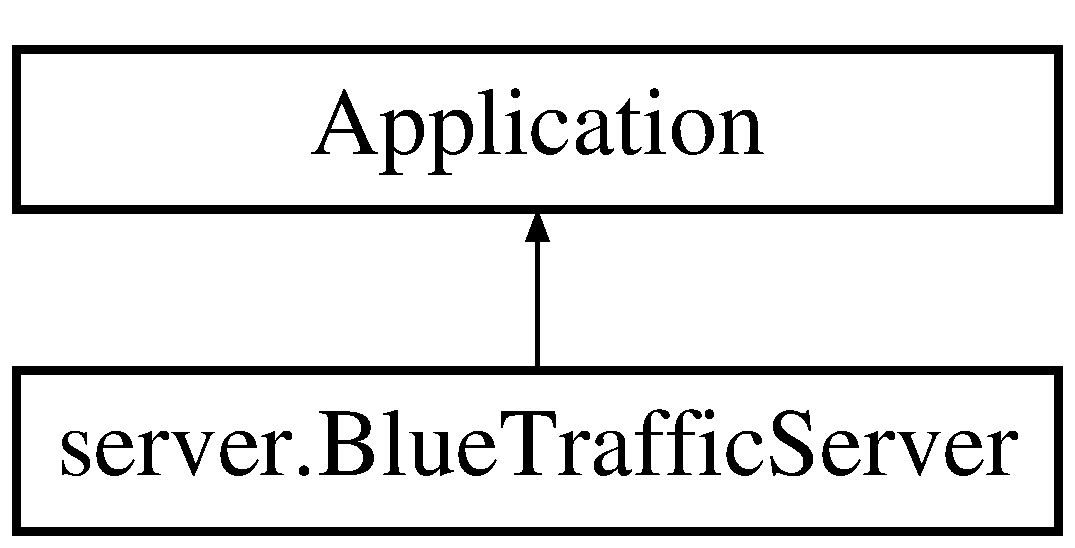
\includegraphics[height=2.000000cm]{classserver_1_1_blue_traffic_server}
\end{center}
\end{figure}
\subsection*{Public Member Functions}
\begin{DoxyCompactItemize}
\item 
void {\bfseries start} (Stage primary\+Stage)\hypertarget{classserver_1_1_blue_traffic_server_a1724087b3c6ced2eb2e1ee84a4742a86}{}\label{classserver_1_1_blue_traffic_server_a1724087b3c6ced2eb2e1ee84a4742a86}

\item 
void {\bfseries init\+Root\+Layout} ()\hypertarget{classserver_1_1_blue_traffic_server_abaa84b680468bf1082782caf8c37d69b}{}\label{classserver_1_1_blue_traffic_server_abaa84b680468bf1082782caf8c37d69b}

\item 
Stage {\bfseries get\+Primary\+Stage} ()\hypertarget{classserver_1_1_blue_traffic_server_a740436c1e9bde88ce9e0f8674a07e7d9}{}\label{classserver_1_1_blue_traffic_server_a740436c1e9bde88ce9e0f8674a07e7d9}

\end{DoxyCompactItemize}
\subsection*{Static Public Member Functions}
\begin{DoxyCompactItemize}
\item 
static void {\bfseries main} (String\mbox{[}$\,$\mbox{]} args)\hypertarget{classserver_1_1_blue_traffic_server_a636d434bdf3fc0615700bcbe65b7a7d8}{}\label{classserver_1_1_blue_traffic_server_a636d434bdf3fc0615700bcbe65b7a7d8}

\end{DoxyCompactItemize}


\subsection{Detailed Description}
This is the main class and it basically doesn\textquotesingle{}t do anything except setting up the window using Java\+FX.

Most of the important stuff is done from the \hyperlink{classserver_1_1_kickstarter}{Kickstarter} class instead of this one. 

The documentation for this class was generated from the following file\+:\begin{DoxyCompactItemize}
\item 
Blue\+Traffic\+Server/src/server/Blue\+Traffic\+Server.\+java\end{DoxyCompactItemize}

\hypertarget{classserver_1_1_client}{}\section{server.\+Client Class Reference}
\label{classserver_1_1_client}\index{server.\+Client@{server.\+Client}}
Inheritance diagram for server.\+Client\+:\begin{figure}[H]
\begin{center}
\leavevmode
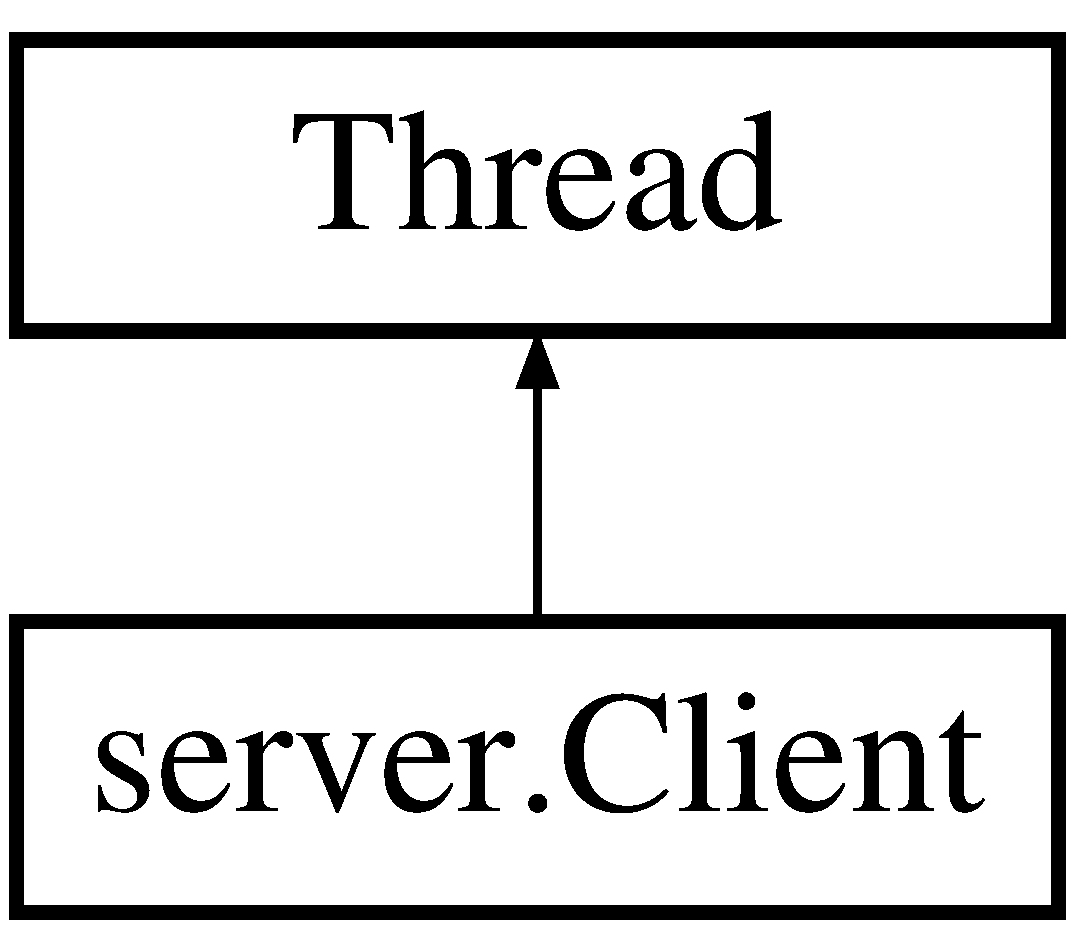
\includegraphics[height=2.000000cm]{classserver_1_1_client}
\end{center}
\end{figure}
\subsection*{Public Member Functions}
\begin{DoxyCompactItemize}
\item 
\hyperlink{classserver_1_1_client_aee63aae8dfec00550d2e2dca453233b8}{Client} (Socket \+\_\+socket)
\item 
String \hyperlink{classserver_1_1_client_a7284190b6acc0b3bba7259386fdc1dae}{get\+IP} ()
\item 
int \hyperlink{classserver_1_1_client_a7007d0065eb9fce43104d0868b480345}{get\+Pos} ()
\item 
boolean \hyperlink{classserver_1_1_client_a372ee497c2b87609e007765b21db53c5}{get\+Walk} ()
\item 
void \hyperlink{classserver_1_1_client_a40f63bbb350bc2f1a65239c04a4a2905}{set\+Pos} (Button b, int i)
\item 
void \hyperlink{classserver_1_1_client_abb9c0d4159442e7618eadebd8c34a2ee}{run} ()
\item 
void \hyperlink{classserver_1_1_client_a87b76abeb1dc06113a33ab759a7f1a2b}{send} (String s)
\item 
void \hyperlink{classserver_1_1_client_a9d49beb9c187a988ba27588038292327}{disconnect} ()
\end{DoxyCompactItemize}


\subsection{Detailed Description}
A unique thread for a client. This thread is listening on the socket for input or output from the client. 

\subsection{Constructor \& Destructor Documentation}
\index{server\+::\+Client@{server\+::\+Client}!Client@{Client}}
\index{Client@{Client}!server\+::\+Client@{server\+::\+Client}}
\subsubsection[{\texorpdfstring{Client(\+Socket \+\_\+socket)}{Client(Socket _socket)}}]{\setlength{\rightskip}{0pt plus 5cm}server.\+Client.\+Client (
\begin{DoxyParamCaption}
\item[{Socket}]{\+\_\+socket}
\end{DoxyParamCaption}
)}\hypertarget{classserver_1_1_client_aee63aae8dfec00550d2e2dca453233b8}{}\label{classserver_1_1_client_aee63aae8dfec00550d2e2dca453233b8}
Default constructor. Sets the socket and the client\textquotesingle{}s IP. 

\subsection{Member Function Documentation}
\index{server\+::\+Client@{server\+::\+Client}!disconnect@{disconnect}}
\index{disconnect@{disconnect}!server\+::\+Client@{server\+::\+Client}}
\subsubsection[{\texorpdfstring{disconnect()}{disconnect()}}]{\setlength{\rightskip}{0pt plus 5cm}void server.\+Client.\+disconnect (
\begin{DoxyParamCaption}
{}
\end{DoxyParamCaption}
)}\hypertarget{classserver_1_1_client_a9d49beb9c187a988ba27588038292327}{}\label{classserver_1_1_client_a9d49beb9c187a988ba27588038292327}
Disconnects the client from the server.


\begin{DoxyItemize}
\item Closes the input/ouput with the server.
\item Removes its own IP from the list of clients in the user interface.
\item Also sets the main thread to join (remove) this client\textquotesingle{}s thread before removing it from the client\+List. 
\end{DoxyItemize}\index{server\+::\+Client@{server\+::\+Client}!get\+IP@{get\+IP}}
\index{get\+IP@{get\+IP}!server\+::\+Client@{server\+::\+Client}}
\subsubsection[{\texorpdfstring{get\+I\+P()}{getIP()}}]{\setlength{\rightskip}{0pt plus 5cm}String server.\+Client.\+get\+IP (
\begin{DoxyParamCaption}
{}
\end{DoxyParamCaption}
)}\hypertarget{classserver_1_1_client_a7284190b6acc0b3bba7259386fdc1dae}{}\label{classserver_1_1_client_a7284190b6acc0b3bba7259386fdc1dae}
Gets the IP of the client. \index{server\+::\+Client@{server\+::\+Client}!get\+Pos@{get\+Pos}}
\index{get\+Pos@{get\+Pos}!server\+::\+Client@{server\+::\+Client}}
\subsubsection[{\texorpdfstring{get\+Pos()}{getPos()}}]{\setlength{\rightskip}{0pt plus 5cm}int server.\+Client.\+get\+Pos (
\begin{DoxyParamCaption}
{}
\end{DoxyParamCaption}
)}\hypertarget{classserver_1_1_client_a7007d0065eb9fce43104d0868b480345}{}\label{classserver_1_1_client_a7007d0065eb9fce43104d0868b480345}
Gets the position of the client. \index{server\+::\+Client@{server\+::\+Client}!get\+Walk@{get\+Walk}}
\index{get\+Walk@{get\+Walk}!server\+::\+Client@{server\+::\+Client}}
\subsubsection[{\texorpdfstring{get\+Walk()}{getWalk()}}]{\setlength{\rightskip}{0pt plus 5cm}boolean server.\+Client.\+get\+Walk (
\begin{DoxyParamCaption}
{}
\end{DoxyParamCaption}
)}\hypertarget{classserver_1_1_client_a372ee497c2b87609e007765b21db53c5}{}\label{classserver_1_1_client_a372ee497c2b87609e007765b21db53c5}
Gets the walk signal boolean of the client. \index{server\+::\+Client@{server\+::\+Client}!run@{run}}
\index{run@{run}!server\+::\+Client@{server\+::\+Client}}
\subsubsection[{\texorpdfstring{run()}{run()}}]{\setlength{\rightskip}{0pt plus 5cm}void server.\+Client.\+run (
\begin{DoxyParamCaption}
{}
\end{DoxyParamCaption}
)}\hypertarget{classserver_1_1_client_abb9c0d4159442e7618eadebd8c34a2ee}{}\label{classserver_1_1_client_abb9c0d4159442e7618eadebd8c34a2ee}
This is the thread\textquotesingle{}s running task and is what is constantly running to check for input.

This will initialize the out and in buffers and wait for any new input until the socket is closed forcefully. If certain input is detected like kill and walk, it\textquotesingle{}ll apply certain commands to either end the method completely, or set the walk flag.

In order to see the commands, it\textquotesingle{}ll need to use the \hyperlink{classserver_1_1_crypto}{Crypto} class to decrypt the information located in the incoming input. \index{server\+::\+Client@{server\+::\+Client}!send@{send}}
\index{send@{send}!server\+::\+Client@{server\+::\+Client}}
\subsubsection[{\texorpdfstring{send(\+String s)}{send(String s)}}]{\setlength{\rightskip}{0pt plus 5cm}void server.\+Client.\+send (
\begin{DoxyParamCaption}
\item[{String}]{s}
\end{DoxyParamCaption}
)}\hypertarget{classserver_1_1_client_a87b76abeb1dc06113a33ab759a7f1a2b}{}\label{classserver_1_1_client_a87b76abeb1dc06113a33ab759a7f1a2b}
Sends a string to the client by encrypting it first and then sending it through the out buffer as long as the output isn\textquotesingle{}t closed. \index{server\+::\+Client@{server\+::\+Client}!set\+Pos@{set\+Pos}}
\index{set\+Pos@{set\+Pos}!server\+::\+Client@{server\+::\+Client}}
\subsubsection[{\texorpdfstring{set\+Pos(\+Button b, int i)}{setPos(Button b, int i)}}]{\setlength{\rightskip}{0pt plus 5cm}void server.\+Client.\+set\+Pos (
\begin{DoxyParamCaption}
\item[{Button}]{b, }
\item[{int}]{i}
\end{DoxyParamCaption}
)}\hypertarget{classserver_1_1_client_a40f63bbb350bc2f1a65239c04a4a2905}{}\label{classserver_1_1_client_a40f63bbb350bc2f1a65239c04a4a2905}
Sets the position of the client. 

The documentation for this class was generated from the following file\+:\begin{DoxyCompactItemize}
\item 
Blue\+Traffic\+Server/src/server/Client.\+java\end{DoxyCompactItemize}

\hypertarget{classserver_1_1_crypto}{}\section{server.\+Crypto Class Reference}
\label{classserver_1_1_crypto}\index{server.\+Crypto@{server.\+Crypto}}
\subsection*{Static Public Member Functions}
\begin{DoxyCompactItemize}
\item 
static String \hyperlink{classserver_1_1_crypto_a3a176b4682bafdfff2db96e7e0930373}{encrypt} (String message, String init\+Vector)
\item 
static String \hyperlink{classserver_1_1_crypto_afe179a0b8528595a0e847105d5d43dbf}{decrypt} (String encrypted, String init\+Vector)
\item 
static String \hyperlink{classserver_1_1_crypto_ab6d2b770608404214a0a9427b5003724}{get\+Random\+IV} ()
\end{DoxyCompactItemize}


\subsection{Detailed Description}
Cryptographic class.

This class is used to decrypt and encrypt the input and output from the server/client using an A\+ES with an 128-\/bit key. It has a symmetrical key as seen below and will use a random generated 16-\/byte IV which is sent with the message to always output different encrypted results every time.

This will ensure that no one will be able to see the different commands sent by the server/client to interact which means no one can act like the server and send the stop command to the clients without being the server with the correctly encrypted commands. 

\subsection{Member Function Documentation}
\index{server\+::\+Crypto@{server\+::\+Crypto}!decrypt@{decrypt}}
\index{decrypt@{decrypt}!server\+::\+Crypto@{server\+::\+Crypto}}
\subsubsection[{\texorpdfstring{decrypt(\+String encrypted, String init\+Vector)}{decrypt(String encrypted, String initVector)}}]{\setlength{\rightskip}{0pt plus 5cm}static String server.\+Crypto.\+decrypt (
\begin{DoxyParamCaption}
\item[{String}]{encrypted, }
\item[{String}]{init\+Vector}
\end{DoxyParamCaption}
)\hspace{0.3cm}{\ttfamily [static]}}\hypertarget{classserver_1_1_crypto_afe179a0b8528595a0e847105d5d43dbf}{}\label{classserver_1_1_crypto_afe179a0b8528595a0e847105d5d43dbf}
Decrypts the input by using the encrypted text and the IV.

Will first decode the IV into a 16-\/byte array and then use the static symmetric key to decrypt the message through A\+ES. \index{server\+::\+Crypto@{server\+::\+Crypto}!encrypt@{encrypt}}
\index{encrypt@{encrypt}!server\+::\+Crypto@{server\+::\+Crypto}}
\subsubsection[{\texorpdfstring{encrypt(\+String message, String init\+Vector)}{encrypt(String message, String initVector)}}]{\setlength{\rightskip}{0pt plus 5cm}static String server.\+Crypto.\+encrypt (
\begin{DoxyParamCaption}
\item[{String}]{message, }
\item[{String}]{init\+Vector}
\end{DoxyParamCaption}
)\hspace{0.3cm}{\ttfamily [static]}}\hypertarget{classserver_1_1_crypto_a3a176b4682bafdfff2db96e7e0930373}{}\label{classserver_1_1_crypto_a3a176b4682bafdfff2db96e7e0930373}
Encrypts input by using the incoming IV and the command.

It uses A\+ES with the static key before returning a Base64 encoded String which makes it easy to decode into bytes again once it is received on the other end. \index{server\+::\+Crypto@{server\+::\+Crypto}!get\+Random\+IV@{get\+Random\+IV}}
\index{get\+Random\+IV@{get\+Random\+IV}!server\+::\+Crypto@{server\+::\+Crypto}}
\subsubsection[{\texorpdfstring{get\+Random\+I\+V()}{getRandomIV()}}]{\setlength{\rightskip}{0pt plus 5cm}static String server.\+Crypto.\+get\+Random\+IV (
\begin{DoxyParamCaption}
{}
\end{DoxyParamCaption}
)\hspace{0.3cm}{\ttfamily [static]}}\hypertarget{classserver_1_1_crypto_ab6d2b770608404214a0a9427b5003724}{}\label{classserver_1_1_crypto_ab6d2b770608404214a0a9427b5003724}
Creates a random IV.

This is used to ensure that the encrypted message is different every single time it is sent. If this wasn\textquotesingle{}t the case it would be easy to see that the same messages are being sent as the encrypted text would be the same every time. 

The documentation for this class was generated from the following file\+:\begin{DoxyCompactItemize}
\item 
Blue\+Traffic\+Server/src/server/Crypto.\+java\end{DoxyCompactItemize}

\hypertarget{classserver_1_1_g_u_i_controller}{}\section{server.\+G\+U\+I\+Controller Class Reference}
\label{classserver_1_1_g_u_i_controller}\index{server.\+G\+U\+I\+Controller@{server.\+G\+U\+I\+Controller}}
\subsection*{Public Member Functions}
\begin{DoxyCompactItemize}
\item 
void \hyperlink{classserver_1_1_g_u_i_controller_acf92ca1ea088749ae09c2b0af80aa1bb}{launch} (Action\+Event event)
\item 
void \hyperlink{classserver_1_1_g_u_i_controller_aa9937074dfbc56bff950e32b50839830}{stop} (Action\+Event event)
\item 
void \hyperlink{classserver_1_1_g_u_i_controller_aae8010b06b7b15549184c337bf52143d}{stop} ()
\item 
void \hyperlink{classserver_1_1_g_u_i_controller_a5d4f06a9637212f2997fac0c4e2170af}{change\+Yellow\+Slider\+Value} (Mouse\+Event event)
\item 
void \hyperlink{classserver_1_1_g_u_i_controller_adf1f5bc21fa366cef67190136b77592d}{change\+Green\+Slider\+Value} (Mouse\+Event event)
\item 
void \hyperlink{classserver_1_1_g_u_i_controller_addab5196eb4594616a3bd2dcc29489db}{change\+Red\+Slider\+Value} (Mouse\+Event event)
\item 
void \hyperlink{classserver_1_1_g_u_i_controller_a6bacbc209aafa62be4804ff3856376e3}{apply\+Colors} (Action\+Event event)
\item 
void \hyperlink{classserver_1_1_g_u_i_controller_a8cd1634fc294643ea4b9521e8208fe47}{sync\+\_\+warning} (Action\+Event event)
\item 
void \hyperlink{classserver_1_1_g_u_i_controller_ae1193dc919447002f2b789250150ca5f}{assign\+Light} (Action\+Event event)
\end{DoxyCompactItemize}
\subsection*{Public Attributes}
\begin{DoxyCompactItemize}
\item 
List\+View$<$ String $>$ {\bfseries list\+\_\+client\+List}\hypertarget{classserver_1_1_g_u_i_controller_a1dcb7f6387529a4b8274c2c899505398}{}\label{classserver_1_1_g_u_i_controller_a1dcb7f6387529a4b8274c2c899505398}

\item 
Image\+View {\bfseries view\+\_\+traffic\+Light1}\hypertarget{classserver_1_1_g_u_i_controller_af75f7c418183ce486b2b86dbd9fc305c}{}\label{classserver_1_1_g_u_i_controller_af75f7c418183ce486b2b86dbd9fc305c}

\item 
Text\+Area {\bfseries log}\hypertarget{classserver_1_1_g_u_i_controller_a776c464bc80de311d3e029f315f0f6c8}{}\label{classserver_1_1_g_u_i_controller_a776c464bc80de311d3e029f315f0f6c8}

\end{DoxyCompactItemize}


\subsection{Detailed Description}
Java\+FX controller. Controls all the buttons, labels, sliders, textareas and such.

Most of the main stuff is contained within the \char`\"{}\+Kickstarter\char`\"{} main thread instead of this one. This will ensure that the \hyperlink{classserver_1_1_g_u_i_controller}{G\+U\+I\+Controller} won\textquotesingle{}t need to listen to any sockets, create any clients or something similar. 

\subsection{Member Function Documentation}
\index{server\+::\+G\+U\+I\+Controller@{server\+::\+G\+U\+I\+Controller}!apply\+Colors@{apply\+Colors}}
\index{apply\+Colors@{apply\+Colors}!server\+::\+G\+U\+I\+Controller@{server\+::\+G\+U\+I\+Controller}}
\subsubsection[{\texorpdfstring{apply\+Colors(\+Action\+Event event)}{applyColors(ActionEvent event)}}]{\setlength{\rightskip}{0pt plus 5cm}void server.\+G\+U\+I\+Controller.\+apply\+Colors (
\begin{DoxyParamCaption}
\item[{Action\+Event}]{event}
\end{DoxyParamCaption}
)}\hypertarget{classserver_1_1_g_u_i_controller_a6bacbc209aafa62be4804ff3856376e3}{}\label{classserver_1_1_g_u_i_controller_a6bacbc209aafa62be4804ff3856376e3}
Applies the colors by getting the frequency from the sliders and sending it to the clients and writes to the log. \index{server\+::\+G\+U\+I\+Controller@{server\+::\+G\+U\+I\+Controller}!assign\+Light@{assign\+Light}}
\index{assign\+Light@{assign\+Light}!server\+::\+G\+U\+I\+Controller@{server\+::\+G\+U\+I\+Controller}}
\subsubsection[{\texorpdfstring{assign\+Light(\+Action\+Event event)}{assignLight(ActionEvent event)}}]{\setlength{\rightskip}{0pt plus 5cm}void server.\+G\+U\+I\+Controller.\+assign\+Light (
\begin{DoxyParamCaption}
\item[{Action\+Event}]{event}
\end{DoxyParamCaption}
)}\hypertarget{classserver_1_1_g_u_i_controller_ae1193dc919447002f2b789250150ca5f}{}\label{classserver_1_1_g_u_i_controller_ae1193dc919447002f2b789250150ca5f}
This is used for all the buttons on the map.

It will first check what button was pressed, whether it\textquotesingle{}s a normal traffic light and then a walking sign button since they are of different icons and sizes. It also sets the button\textquotesingle{}s icon, and sends arguments like what client is selected to the assign\+Light method. \index{server\+::\+G\+U\+I\+Controller@{server\+::\+G\+U\+I\+Controller}!change\+Green\+Slider\+Value@{change\+Green\+Slider\+Value}}
\index{change\+Green\+Slider\+Value@{change\+Green\+Slider\+Value}!server\+::\+G\+U\+I\+Controller@{server\+::\+G\+U\+I\+Controller}}
\subsubsection[{\texorpdfstring{change\+Green\+Slider\+Value(\+Mouse\+Event event)}{changeGreenSliderValue(MouseEvent event)}}]{\setlength{\rightskip}{0pt plus 5cm}void server.\+G\+U\+I\+Controller.\+change\+Green\+Slider\+Value (
\begin{DoxyParamCaption}
\item[{Mouse\+Event}]{event}
\end{DoxyParamCaption}
)}\hypertarget{classserver_1_1_g_u_i_controller_adf1f5bc21fa366cef67190136b77592d}{}\label{classserver_1_1_g_u_i_controller_adf1f5bc21fa366cef67190136b77592d}
Changes the label where the green slider is to show its value. \index{server\+::\+G\+U\+I\+Controller@{server\+::\+G\+U\+I\+Controller}!change\+Red\+Slider\+Value@{change\+Red\+Slider\+Value}}
\index{change\+Red\+Slider\+Value@{change\+Red\+Slider\+Value}!server\+::\+G\+U\+I\+Controller@{server\+::\+G\+U\+I\+Controller}}
\subsubsection[{\texorpdfstring{change\+Red\+Slider\+Value(\+Mouse\+Event event)}{changeRedSliderValue(MouseEvent event)}}]{\setlength{\rightskip}{0pt plus 5cm}void server.\+G\+U\+I\+Controller.\+change\+Red\+Slider\+Value (
\begin{DoxyParamCaption}
\item[{Mouse\+Event}]{event}
\end{DoxyParamCaption}
)}\hypertarget{classserver_1_1_g_u_i_controller_addab5196eb4594616a3bd2dcc29489db}{}\label{classserver_1_1_g_u_i_controller_addab5196eb4594616a3bd2dcc29489db}
Changes the label where the red slider is to show its value. \index{server\+::\+G\+U\+I\+Controller@{server\+::\+G\+U\+I\+Controller}!change\+Yellow\+Slider\+Value@{change\+Yellow\+Slider\+Value}}
\index{change\+Yellow\+Slider\+Value@{change\+Yellow\+Slider\+Value}!server\+::\+G\+U\+I\+Controller@{server\+::\+G\+U\+I\+Controller}}
\subsubsection[{\texorpdfstring{change\+Yellow\+Slider\+Value(\+Mouse\+Event event)}{changeYellowSliderValue(MouseEvent event)}}]{\setlength{\rightskip}{0pt plus 5cm}void server.\+G\+U\+I\+Controller.\+change\+Yellow\+Slider\+Value (
\begin{DoxyParamCaption}
\item[{Mouse\+Event}]{event}
\end{DoxyParamCaption}
)}\hypertarget{classserver_1_1_g_u_i_controller_a5d4f06a9637212f2997fac0c4e2170af}{}\label{classserver_1_1_g_u_i_controller_a5d4f06a9637212f2997fac0c4e2170af}
Changes the label where the yellow slider is to show its value. \index{server\+::\+G\+U\+I\+Controller@{server\+::\+G\+U\+I\+Controller}!launch@{launch}}
\index{launch@{launch}!server\+::\+G\+U\+I\+Controller@{server\+::\+G\+U\+I\+Controller}}
\subsubsection[{\texorpdfstring{launch(\+Action\+Event event)}{launch(ActionEvent event)}}]{\setlength{\rightskip}{0pt plus 5cm}void server.\+G\+U\+I\+Controller.\+launch (
\begin{DoxyParamCaption}
\item[{Action\+Event}]{event}
\end{DoxyParamCaption}
)}\hypertarget{classserver_1_1_g_u_i_controller_acf92ca1ea088749ae09c2b0af80aa1bb}{}\label{classserver_1_1_g_u_i_controller_acf92ca1ea088749ae09c2b0af80aa1bb}
Event triggered by button\+\_\+start.

This will create a new thread which will make app\+Starter a new \hyperlink{classserver_1_1_kickstarter}{Kickstarter} object and send arguments. It will then start the thread, and disable the start button, while enabling the stop button. \index{server\+::\+G\+U\+I\+Controller@{server\+::\+G\+U\+I\+Controller}!stop@{stop}}
\index{stop@{stop}!server\+::\+G\+U\+I\+Controller@{server\+::\+G\+U\+I\+Controller}}
\subsubsection[{\texorpdfstring{stop(\+Action\+Event event)}{stop(ActionEvent event)}}]{\setlength{\rightskip}{0pt plus 5cm}void server.\+G\+U\+I\+Controller.\+stop (
\begin{DoxyParamCaption}
\item[{Action\+Event}]{event}
\end{DoxyParamCaption}
)}\hypertarget{classserver_1_1_g_u_i_controller_aa9937074dfbc56bff950e32b50839830}{}\label{classserver_1_1_g_u_i_controller_aa9937074dfbc56bff950e32b50839830}
Event triggered by button\+\_\+stop.

See \hyperlink{classserver_1_1_g_u_i_controller_aae8010b06b7b15549184c337bf52143d}{stop()} for details. \index{server\+::\+G\+U\+I\+Controller@{server\+::\+G\+U\+I\+Controller}!stop@{stop}}
\index{stop@{stop}!server\+::\+G\+U\+I\+Controller@{server\+::\+G\+U\+I\+Controller}}
\subsubsection[{\texorpdfstring{stop()}{stop()}}]{\setlength{\rightskip}{0pt plus 5cm}void server.\+G\+U\+I\+Controller.\+stop (
\begin{DoxyParamCaption}
{}
\end{DoxyParamCaption}
)}\hypertarget{classserver_1_1_g_u_i_controller_aae8010b06b7b15549184c337bf52143d}{}\label{classserver_1_1_g_u_i_controller_aae8010b06b7b15549184c337bf52143d}
Kills the app\+Starter and its thread. Reenables the start button. \index{server\+::\+G\+U\+I\+Controller@{server\+::\+G\+U\+I\+Controller}!sync\+\_\+warning@{sync\+\_\+warning}}
\index{sync\+\_\+warning@{sync\+\_\+warning}!server\+::\+G\+U\+I\+Controller@{server\+::\+G\+U\+I\+Controller}}
\subsubsection[{\texorpdfstring{sync\+\_\+warning(\+Action\+Event event)}{sync_warning(ActionEvent event)}}]{\setlength{\rightskip}{0pt plus 5cm}void server.\+G\+U\+I\+Controller.\+sync\+\_\+warning (
\begin{DoxyParamCaption}
\item[{Action\+Event}]{event}
\end{DoxyParamCaption}
)}\hypertarget{classserver_1_1_g_u_i_controller_a8cd1634fc294643ea4b9521e8208fe47}{}\label{classserver_1_1_g_u_i_controller_a8cd1634fc294643ea4b9521e8208fe47}
Shows the warning for desynchronizing the red and green colors and disables it from appearing again during that run. 

The documentation for this class was generated from the following file\+:\begin{DoxyCompactItemize}
\item 
Blue\+Traffic\+Server/src/server/G\+U\+I\+Controller.\+java\end{DoxyCompactItemize}

\hypertarget{classserver_1_1_kickstarter}{}\section{server.\+Kickstarter Class Reference}
\label{classserver_1_1_kickstarter}\index{server.\+Kickstarter@{server.\+Kickstarter}}
Inheritance diagram for server.\+Kickstarter\+:\begin{figure}[H]
\begin{center}
\leavevmode
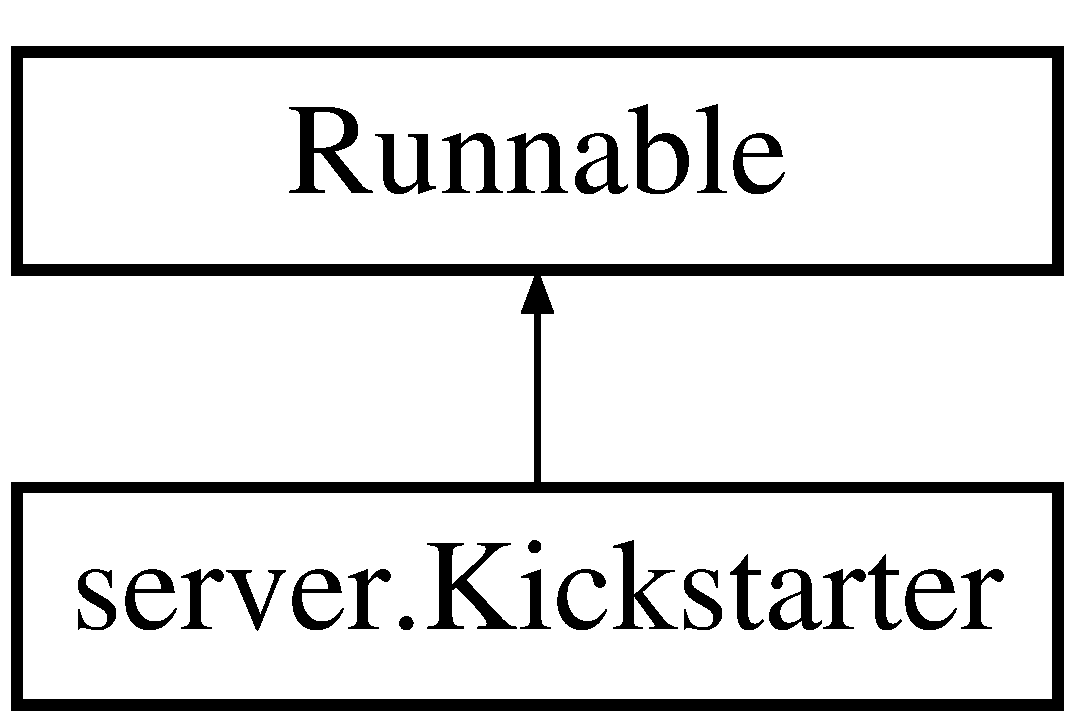
\includegraphics[height=2.000000cm]{classserver_1_1_kickstarter}
\end{center}
\end{figure}
\subsection*{Public Member Functions}
\begin{DoxyCompactItemize}
\item 
\hyperlink{classserver_1_1_kickstarter_a07a921c9b5b248b6c696fd84022126cc}{Kickstarter} (List\+View$<$ String $>$ \+\_\+list\+\_\+client\+List, int arg\+Port, Text\+Area \+\_\+log)  throws I\+O\+Exception
\item 
void \hyperlink{classserver_1_1_kickstarter_ab6d66e280ed60dafe8ca1f7b7d63b21e}{run} ()
\item 
void \hyperlink{classserver_1_1_kickstarter_a1b0a95c249c2e13bcc6218e3e24b3f29}{set\+Frequency} (int color, int frequency)
\item 
void \hyperlink{classserver_1_1_kickstarter_af04e25f1ce0ef4920bb044f0a0ad8b78}{synchronize\+Clients} ()
\item 
void \hyperlink{classserver_1_1_kickstarter_a5842570621b483e05c31d05fa593ee4a}{kill} ()
\item 
boolean \hyperlink{classserver_1_1_kickstarter_ac3e3c0348f02cc1a08cfa49a7990491d}{assign\+Light} (Button b, int list, int pos, boolean walk)
\end{DoxyCompactItemize}
\subsection*{Static Public Member Functions}
\begin{DoxyCompactItemize}
\item 
static void \hyperlink{classserver_1_1_kickstarter_ab976bbeaa74e2b6a9b61126707df9140}{log} (String t)
\end{DoxyCompactItemize}
\subsection*{Public Attributes}
\begin{DoxyCompactItemize}
\item 
boolean {\bfseries is\+Running}\hypertarget{classserver_1_1_kickstarter_a184746683b94fbb9b35d09597fed892e}{}\label{classserver_1_1_kickstarter_a184746683b94fbb9b35d09597fed892e}

\end{DoxyCompactItemize}
\subsection*{Static Public Attributes}
\begin{DoxyCompactItemize}
\item 
static Text\+Area {\bfseries log}\hypertarget{classserver_1_1_kickstarter_ae8a852a9e388b350610fad0f51178ab6}{}\label{classserver_1_1_kickstarter_ae8a852a9e388b350610fad0f51178ab6}

\item 
static List\+View$<$ String $>$ {\bfseries list\+\_\+client\+List}\hypertarget{classserver_1_1_kickstarter_ac9e598cda0986ee51231eb6b6bcd084f}{}\label{classserver_1_1_kickstarter_ac9e598cda0986ee51231eb6b6bcd084f}

\item 
static List$<$ \hyperlink{classserver_1_1_client}{Client} $>$ {\bfseries client\+List}\hypertarget{classserver_1_1_kickstarter_a841d1ef40496a543ee9319983884fd07}{}\label{classserver_1_1_kickstarter_a841d1ef40496a543ee9319983884fd07}

\item 
static List$<$ String $>$ {\bfseries applicable\+List}\hypertarget{classserver_1_1_kickstarter_a6ed3fe0b4d90f3de3b315bcb70ea89e1}{}\label{classserver_1_1_kickstarter_a6ed3fe0b4d90f3de3b315bcb70ea89e1}

\end{DoxyCompactItemize}


\subsection{Detailed Description}
This class is meant as a main method thread where lists, sockets and other information is initialized and taken care of. It is basically a bridge between the \hyperlink{classserver_1_1_g_u_i_controller}{G\+U\+I\+Controller} and the respective clients. This ensures that the \hyperlink{classserver_1_1_g_u_i_controller}{G\+U\+I\+Controller} won\textquotesingle{}t need to have the list fields, nor need to create new clients or listen to the socket for new incoming clients.

This class also synchronizes all clients, and will send a kill command to them if the server is abruptly stopped. 

\subsection{Constructor \& Destructor Documentation}
\index{server\+::\+Kickstarter@{server\+::\+Kickstarter}!Kickstarter@{Kickstarter}}
\index{Kickstarter@{Kickstarter}!server\+::\+Kickstarter@{server\+::\+Kickstarter}}
\subsubsection[{\texorpdfstring{Kickstarter(\+List\+View$<$ String $>$ \+\_\+list\+\_\+client\+List, int arg\+Port, Text\+Area \+\_\+log)}{Kickstarter(ListView< String > _list_clientList, int argPort, TextArea _log)}}]{\setlength{\rightskip}{0pt plus 5cm}server.\+Kickstarter.\+Kickstarter (
\begin{DoxyParamCaption}
\item[{List\+View$<$ String $>$}]{\+\_\+list\+\_\+client\+List, }
\item[{int}]{arg\+Port, }
\item[{Text\+Area}]{\+\_\+log}
\end{DoxyParamCaption}
) throws I\+O\+Exception}\hypertarget{classserver_1_1_kickstarter_a07a921c9b5b248b6c696fd84022126cc}{}\label{classserver_1_1_kickstarter_a07a921c9b5b248b6c696fd84022126cc}
Default constructor and main method.

Will set all parameters to their respective variables. Will also create a listener on the list of clients. 

\subsection{Member Function Documentation}
\index{server\+::\+Kickstarter@{server\+::\+Kickstarter}!assign\+Light@{assign\+Light}}
\index{assign\+Light@{assign\+Light}!server\+::\+Kickstarter@{server\+::\+Kickstarter}}
\subsubsection[{\texorpdfstring{assign\+Light(\+Button b, int list, int pos, boolean walk)}{assignLight(Button b, int list, int pos, boolean walk)}}]{\setlength{\rightskip}{0pt plus 5cm}boolean server.\+Kickstarter.\+assign\+Light (
\begin{DoxyParamCaption}
\item[{Button}]{b, }
\item[{int}]{list, }
\item[{int}]{pos, }
\item[{boolean}]{walk}
\end{DoxyParamCaption}
)}\hypertarget{classserver_1_1_kickstarter_ac3e3c0348f02cc1a08cfa49a7990491d}{}\label{classserver_1_1_kickstarter_ac3e3c0348f02cc1a08cfa49a7990491d}
This will active once a button is pressed on the map tab.

It will assign a map position for the client and its button. It will then log it and synchronize all the clients to ensure they are all on the same page. This will thus change their synchronization depending on where they stand on the map. \index{server\+::\+Kickstarter@{server\+::\+Kickstarter}!kill@{kill}}
\index{kill@{kill}!server\+::\+Kickstarter@{server\+::\+Kickstarter}}
\subsubsection[{\texorpdfstring{kill()}{kill()}}]{\setlength{\rightskip}{0pt plus 5cm}void server.\+Kickstarter.\+kill (
\begin{DoxyParamCaption}
{}
\end{DoxyParamCaption}
)}\hypertarget{classserver_1_1_kickstarter_a5842570621b483e05c31d05fa593ee4a}{}\label{classserver_1_1_kickstarter_a5842570621b483e05c31d05fa593ee4a}
Kills all client threads by killing the \char`\"{}is\+Running\char`\"{} part of \hyperlink{classserver_1_1_kickstarter_ab6d66e280ed60dafe8ca1f7b7d63b21e}{run()}.

This is used to tell all clients that the server is shutting down and will no longer respond. \index{server\+::\+Kickstarter@{server\+::\+Kickstarter}!log@{log}}
\index{log@{log}!server\+::\+Kickstarter@{server\+::\+Kickstarter}}
\subsubsection[{\texorpdfstring{log(\+String t)}{log(String t)}}]{\setlength{\rightskip}{0pt plus 5cm}static void server.\+Kickstarter.\+log (
\begin{DoxyParamCaption}
\item[{String}]{t}
\end{DoxyParamCaption}
)\hspace{0.3cm}{\ttfamily [static]}}\hypertarget{classserver_1_1_kickstarter_ab976bbeaa74e2b6a9b61126707df9140}{}\label{classserver_1_1_kickstarter_ab976bbeaa74e2b6a9b61126707df9140}
Logs by appending to the log textarea in the application.

Is static here instead of \hyperlink{classserver_1_1_g_u_i_controller}{G\+U\+I\+Controller} due to Java\+FX generated variables should not and cannot be static. \index{server\+::\+Kickstarter@{server\+::\+Kickstarter}!run@{run}}
\index{run@{run}!server\+::\+Kickstarter@{server\+::\+Kickstarter}}
\subsubsection[{\texorpdfstring{run()}{run()}}]{\setlength{\rightskip}{0pt plus 5cm}void server.\+Kickstarter.\+run (
\begin{DoxyParamCaption}
{}
\end{DoxyParamCaption}
)}\hypertarget{classserver_1_1_kickstarter_ab6d66e280ed60dafe8ca1f7b7d63b21e}{}\label{classserver_1_1_kickstarter_ab6d66e280ed60dafe8ca1f7b7d63b21e}
As long as the \char`\"{}is\+Running\char`\"{} boolean is true, the server will listen on the port for clients who want to respond. Once the server accepts a client, it\textquotesingle{}ll add it to the client\+List where the listener will pick it up and add it to the list of clients. From here, the client will have its own thread where it can communicate with the server. \index{server\+::\+Kickstarter@{server\+::\+Kickstarter}!set\+Frequency@{set\+Frequency}}
\index{set\+Frequency@{set\+Frequency}!server\+::\+Kickstarter@{server\+::\+Kickstarter}}
\subsubsection[{\texorpdfstring{set\+Frequency(int color, int frequency)}{setFrequency(int color, int frequency)}}]{\setlength{\rightskip}{0pt plus 5cm}void server.\+Kickstarter.\+set\+Frequency (
\begin{DoxyParamCaption}
\item[{int}]{color, }
\item[{int}]{frequency}
\end{DoxyParamCaption}
)}\hypertarget{classserver_1_1_kickstarter_a1b0a95c249c2e13bcc6218e3e24b3f29}{}\label{classserver_1_1_kickstarter_a1b0a95c249c2e13bcc6218e3e24b3f29}
Sends the new light frequencies to all lights. \index{server\+::\+Kickstarter@{server\+::\+Kickstarter}!synchronize\+Clients@{synchronize\+Clients}}
\index{synchronize\+Clients@{synchronize\+Clients}!server\+::\+Kickstarter@{server\+::\+Kickstarter}}
\subsubsection[{\texorpdfstring{synchronize\+Clients()}{synchronizeClients()}}]{\setlength{\rightskip}{0pt plus 5cm}void server.\+Kickstarter.\+synchronize\+Clients (
\begin{DoxyParamCaption}
{}
\end{DoxyParamCaption}
)}\hypertarget{classserver_1_1_kickstarter_af04e25f1ce0ef4920bb044f0a0ad8b78}{}\label{classserver_1_1_kickstarter_af04e25f1ce0ef4920bb044f0a0ad8b78}
Synchronizes all the clients by sending each client a \textquotesingle{}sync0\textquotesingle{} or \textquotesingle{}sync2\textquotesingle{} command. The numbers at the end of these commands corresponds to which lane they\textquotesingle{}re supposed to synchronize with.

The thread will then sleep for around a second to ensure that all the clients are done cancelling their jobs and ready to start over again. After that second has passed, it\textquotesingle{}ll send all the clients a \textquotesingle{}restart\textquotesingle{} command and they\textquotesingle{}ll all end their loops and begin anew simultaneously. 

The documentation for this class was generated from the following file\+:\begin{DoxyCompactItemize}
\item 
Blue\+Traffic\+Server/src/server/Kickstarter.\+java\end{DoxyCompactItemize}

%--- End generated contents ---

% Index
\backmatter
\newpage
\phantomsection
\clearemptydoublepage
\addcontentsline{toc}{chapter}{Index}
\printindex

\end{document}
